\documentclass[letterpaper,12pt]{article}
\usepackage[utf8]{inputenc}
\usepackage[margin=0.8in]{geometry}
\usepackage{graphicx}
\usepackage{listings}
\usepackage[breaklinks]{hyperref}
\usepackage[dvipsnames,todonotes]{xcolor}
\usepackage{todonotes}
\usepackage{float}
\usepackage{booktabs}
\usepackage{csquotes}
\usepackage[style=numeric,backend=biber]{biblatex}
\addbibresource{references.bib}

% \setcounter{section}{-1}

\usepackage{helvet}
\lstset{backgroundcolor = \color{black},
    basicstyle=\ttfamily\footnotesize\color{Cerulean},
    keywordstyle=\bfseries,
    breaklines=true,
    postbreak=\mbox{\textcolor{Rhodamine}{$\hookrightarrow$}\space}
}

\begin{document}
\begin{titlepage}

\newcommand{\HRule}{\rule{\linewidth}{0.5mm}}

\begin{center}

\includegraphics[width=\linewidth]{Images/uvaeng}\\[2.5cm]
\textsc{\Large MSc Security and Network Engineering}\\[0.2cm]
\textsc{\Large Research Project II}\\[0.5cm] 

\HRule \\[0.4cm]
{\huge \bfseries Sharing digital objects using NDN: PID interoperability, planning and scaling}\\[0.4cm]
\HRule \\[0.5cm]
 
by\\[0.2cm]
\textsc{\Large Kees de Jong \& Anas Younis}\\[0.2cm]

{\Large \today}\\[1cm]

\vfill

\end{center}
\end{titlepage}

\tableofcontents
\clearpage

\begin{abstract}
Research clouds contain diverse and large datasets, this data is published by the use of \glspl{pid}. The current paradigm utilizes data transmissions by the means of host-to-host connections (IP), where every data request from the consumer is answered with a data transfer from the source (the producer). This approach can potentially cause congestion and delays with many data consumers. \gls{ndn} is a data centric approach where unique data, once requested, is stored on intermediate hops in the network. Consecutive requests for that unique data object are then made available by these intermediate hops (caching). This approach distributes traffic load more efficient and reliable compared to host-to-host connection oriented techniques \cite{ndn-ccr}. Furthermore, one of the most important technical challenges is to incorporate interoperability between\gls{ndn} and the different \gls{pid} naming schemas. These naming schemas are used by data providers within these data infrastructures for sharing and identifying digital objects. This research investigated how identification services and transmission services can be better integrated by the use of \gls{ndn}. In order to create this integration, a translation between the different naming schemas was developed and made extendable for future \gls{pid} types. Furthermore, a method was researched and applied for planning and scaling an \gls{ndn} with scalability in mind.
\end{abstract}

% The work you did with NDN/PID is to investigate how identification services and transmission services can be better integrated. The current world: PID is publication, and transmission is based on other network protocols. Our motivtion is to investigate if PID, caching, digital object discovery, routine etc. can be all implemented using the\gls{ndn} technology





%SeaDataCloud is a distributed infrastructure to manage large and diverse sets of data about seas and oceans. This Pan-European network offers data access to support scientific workflows which varies from climate change prediction to offshore engineering \cite{sdc}.
%Different independent organizations push data into this infrastructure which are then automatically and manually curated to ensure correct data formats. A \gls{pid} is then assigned when it’s stored in the catalog. This \gls{pid} ensures that the data can be identified, independent of its location in the infrastructure \cite{icn-survey, icn-bd}. 
%CS3 is another case of a data infrastructure, which includes around hundred institutions and companies from around the world and this number keeps growing.
%Their most important technical challenge is incorporating introperability of the different naming schemas being used within CS3.
\section{Introduction}
% Short abstract introduction here about this section (can be done when finished)

\subsection{Background}
\label{introduction-background}
% What is SeaDataCloud's exact problem? Make the problem clear so that our solution fits the problem. Try to look at it from all angles, like an os3 teacher would

% European Open Science Cloud
Research clouds such as proposed in the \gls{eosc} will offer Europe's 1.7 million researchers and 70 million science and technology professionals the means to store, share and re-use large volumes of information generated by the big data revolution \cite{eurocloud}. Research clouds publish datasets from distributed sources, identified by a \gls{pid} (more details in section \ref{pid-intr}). These datasets are not accessed via e.g. a simple web portal like traditional internet objects on the web. Instead these requests are processed by e.g. a data catalog of the federated research cloud. Therefore, research clouds face the challenge of identifying distributed data in a federated cloud, provide data provenance and provide a scalable service to serve many users that request large datasets.

Furthermore, research clouds face a trend of increased data production and consumption, which is expected to grow. This general trend in research clouds calls for a data distribution solution that better supports the scale and complexity. In this section we will briefly discuss the technical challenges.

An example of such a research cloud is SeaDataNet, which is a distributed marine data infrastructure network for managing the large and diverse data sets collected by the oceanographic fleets and the automatic observation systems. SeaDataNet started the SeaDataCloud project in 2016. Their aim is to advance and increase the usage of SeaDataNet's services by adopting cloud and high performance computing technology for better performance \cite{sdc}. Their current infrastructure is a centralized solution (figure \ref{fig:sdc_cur}), as the current cache is a central catalogue which duplicates the entire data repository.

\begin{figure}[H]
\centering
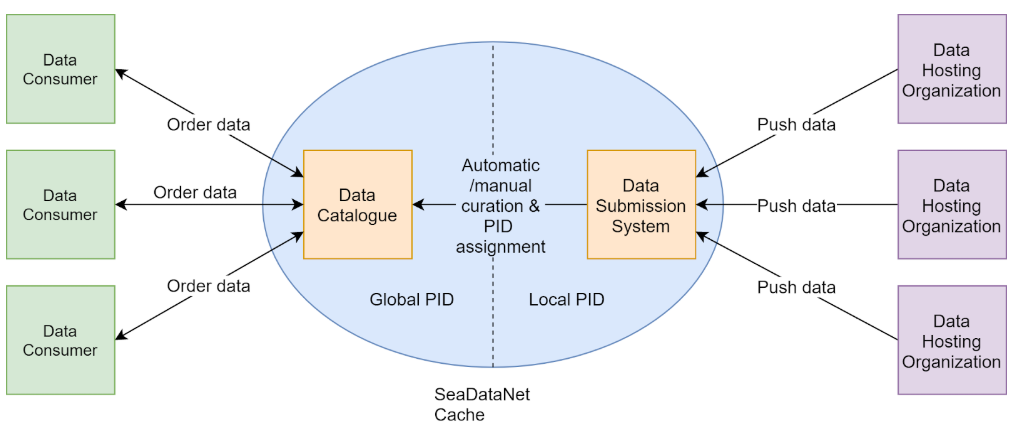
\includegraphics[scale=0.57]{Images/SDC_current.png}
\caption{SeaDataCloud's current infrastructure.}
\label{fig:sdc_cur}
\end{figure}

Data consumers use host-to-host-connections (IP) to pull data from this cache, which could cause congestion with many concurrent data consumers. SeaDataCloud aims at considerably advancing SeaDataNet services and increasing their usage, more users are expected to be engaged and for longer sessions \cite{sdc-eu}.
 
Another research cloud example is CS3, which is a data infrastructure that brings together users, researchers, developers, technology, and service providers of on-premise cloud services as well as large cloud service companies \cite{cs3}. The \gls{cs3} community has been growing for the last three years and currently includes around one hundred institutions and companies from around the world.

The general problem that can be subtracted from figure \ref{fig:sdc_cur} is that research clouds face a potential congestion problem, and thus network and data processing performance degradation when many concurrent data consumers are active. In the field of big science (big data), several data distribution technologies are being experimented with, one of these technologies is \gls{ndn} (more details in section \ref{introduction-ndn}). \gls{ndn} could be a solution to distribute network load and data distribution more efficiently.

% feedback below partially applied, check again
% You should highlight: i) research data infrastructure publishes data from distributed sources, but serve large user communities, ii) such data infrastructure is not a simple web portal of accessing digital objects, but federation of data catalog, repositories and other processing services, iii) research data face challenges of identification, provenance, workflows etc,; the data in the infrastructure is continuously updated, sometimes also from the user. 

% One of the technical challenges is the distribution of the data across the communities. The issue is that the data is distributed by different data providers across these communities, each with their own naming schema. Therefore, interoperability across different naming schemas has to be achieved. Users should be able to request data across these communities, without having to cope with different schemas for data they request. Another technical challenge is to serve this data to a large number of users. 

% The current approach can potentially cause congestion and delays with many concurrent users consuming data from the highlighted distributed data infrastructures. On top of that, the large number of users is still growing. In section \ref{tech-oview} we highlight state of the art technologies to deal with these challenges. We will create a design which achieves interoperability across different naming schemas and alleviates network latency and congestion.

% stuff below is not true i suppose, this interoperability only becomes an issue when ndn is introduced. pid schemas work just fine together.
% One of the most important topics and technical challenge of \gls{cs3} services is interoperability of the different naming schemes being used to identify data. Development of interoperability protocols is important to provide data sharing capabilities for all users across all institutions in the field of education and research.

\subsection{Research question}
\label{introduction-research-question}
% Based on the use case and related work, what is it that we will research and why? What is it that we want to answer?
With the technical challenges and problem statement in mind, as described in section \ref{introduction-background}, we will answer the following questions which are divided into two main research questions.

\begin{enumerate}
	\item A translation is needed between the \gls{pid} and \gls{ndn} namespace in order to make these solutions compatible, thus; how to make the \gls{pid} and \gls{ndn} namespace interoperable?
\end{enumerate}

We will research different \gls{pid} types to find a feasible approach to implement \gls{ndn} interoperability with extensibility in mind for \gls{pid} types.

%This is in response to the highlighted data infrastructures described in section \ref{introduction-background}, which cope with interoperability across different data providers. This is due to the fact that the different data providers use different naming schema to serve objects to data consumers.

%Next to this, SeaDataCloud's planned solution needs to support multiple \gls{pid} types, as \glspl{pid} that get assigned to objects in their infrastructure can be of any type, we will look into supporting different \gls{pid} types to find a feasible solution to implement future \gls{pid} types easily. This will be answered with the following sub-questions.
\begin{itemize}
    \item[--] How to support different \gls{pid} types?
    \item[--] How to incorporate extensibility for future \gls{pid} schemas?
\end{itemize}

The problem statement discussed in \ref{introduction-background} calls for a data distribution solution. Therefore, we will research the planning and deployment of an \gls{ndn} with scalability in mind. To achieve this, the following research question needs to be answered.
\begin{enumerate}
\setcounter{enumi}{1}
    \item How to plan and manage an \gls{ndn}'s life cycle with scalability in mind?
\end{enumerate}

To answer this research question we need to analyze the known scalability problems in \gls{ndn}. Furthermore, the term scalability needs to apply to manageability as well. If scaling in or out in terms of resources is made uncomplicated, the efforts needed to manage this infrastructure needs to stay the same.
\begin{itemize}
    \item[--] Which \gls{ndn} scaling problems are known?
    \item[--] Which method can be used to plan an NDN?
    \item[--] How to deploy an \gls{ndn} with scalability in mind?
\end{itemize}

\subsection{Scope}
\label{introduction-scope}
% What will we do and what will we skip? Based on what's already done in related work and our research question

% related work (section \ref{introduction-related-work}) and

Based on the research question we defined the following scope. We will develop a method to make the \gls{pid} types \gls{urn}, Handle and \gls{doi} interoperable with the \gls{ndn} namespace. This will be done to demonstrate that interoperability of different \gls{pid} types is possible within \gls{ndn}. The reason we do not cover more \gls{pid} types in our methodology is because with the aforementioned \gls{pid} types we can already prove that \gls{pid} interoperability is possible. Therefore, the interoperability goals are to demonstrate that different \gls{pid} types can be used within \gls{ndn}.

The planning of the \gls{ndn} has the following goals. We did not have access to performance monitoring data from research clouds such as SeaDataCloud or CS3. Thus, a starting baseline will be determined based on the known performance limitations (section \ref{introduction-related-work-ndn}) and the problem statement discussed in section \ref{introduction-background}. Using this starting baseline, a method will be developed for \gls{ndn} planning and deployment. This includes a proof of concept where, based on \gls{ndn}'s adaptability, the network can be adjusted for scale in both performance but also in terms of manageability. The proof of concept will be limited to existing software solutions. Therefore, solutions that are still in a research or development phase and not yet implemented or made public will not be explored in the proof of concept. The proof of concept will be setup in a small scale and is used to demonstrate the methods and train of thought used to deploy the \gls{ndn} with the mentioned scalability properties. However, the methods developed should be applicable to also larger deployments (research clouds) without alternation.

\subsection{Report structure}
This report is structured as follows; after the background of this research is discussed, the research questions are presented. This research is divided into two research parts, each with their own scope and results. Related work will be discussed in section \ref{introduction-related-work}. A technical background is provided in section \ref{tech-oview}. These technical details assist in understanding our methods and technology choices we made to answer the research questions. These technologies are used in our methodology sections; \ref{pid-poc} and \ref{planning-ndn}. These methods are tested in a proof of concept. The results of both methods in the proof of concept will be summarized and the novelty evaluated in the discussion (section \ref{disc}). Furthermore, we also discuss preliminary performance results based on our proof of concept in section \ref{discussion-performance}. We will conclude our findings and provide future work in section \ref{fut}. Uncommon acronyms are listed in the appendix in section \ref{appendix}.



% After introducing the concepts and related work of our research subjects, we will continue to discuss the technical background in section \ref{tech-oview}. In this technical background we will explore \glspl{pid}, \gls{ndn}, McCabe, \gls{tosca} and virtualization in more detail with the research scope in mind.  Our methodology in sections \ref{pid-poc} and \ref{planning-ndn} provide a prototype for demonstrating the planning and scaling of an \gls{ndn} with \gls{pid} interoperability. For \gls{pid} interoperability with the \gls{ndn} namespace we will also focus on the ease of extensibility for future \gls{pid} types. Our interoperability approach is integrated in our proof of concept which makes use of the planning and scaling methods of section \ref{planning-ndn}. By combining these methods we will be able to demonstrate that the consumer can still retrieve objects from the producer, despite scaling the \gls{ndn} in our out. And thus provides data distribution by the use of \gls{ndn}, which in turn lowers the chance of network congestion for e.g. research clouds. Furthermore, we will discuss our combined methods in more detail in section \ref{disc}, where 

\section{State of the art}
\label{tech-oview}
% most recent stage in the development of a product, incorporating the newest ideas and features
% add discussion about these tech in introduction or conclusion of this section
% Analyze the requirement for your research questions

In this section we provide an overview of the technologies used in our methodology sections \ref{pid-poc} and \ref{planning-ndn}.

\subsection{PID types and naming schema}\label{pid-types}
Over the years, different kinds of PIDs have emerged. The most widely used PID types are Handle (first major PID type introduced in 1994), DOI, PURL, URN and ARK \cite{pid-oview, odin, hdl}. For our proof of concept described in section \ref{pid-poc}, we will describe Handle, DOI and URN. For a technical overview of the aforementioned PID types we refer to the research done by Karakannas \cite{icn-bd}. 

The most widely used PID types make use of the same hierarchical naming schema, which starts with a PID type identifier such as \texttt{"urn"}, \texttt{"handle"} or \texttt{"doi"}, followed by some kind of delimiter. The PID type identifier is usually embedded in the URL of the PID resolver naming authority. Such as \texttt{"http://hdl.handle.net/"} for resolving Handle PIDs, \texttt{"https://doi.pangaea.de/"} for resolving DOI PIDs or \texttt{"http://resolver.kb.nl/resolve?urn="} for resolving URN PIDs, followed by the PID of the digital object. This means that PIDs are usually associated with a resolver via a URL \cite{ids, icn-bd}. A PID web resolver redirects to the location of the digital object. After the first delimiter, the naming authority is defined (this can be seen as a prefix of a digital object), followed again by some kind of delimiter. Finally there is a specific string for indicating the namespace, which is the identity of a digital object within the naming authority. Table \ref{tab:pid} below shows an overview of the mentioned PID types. 
%For a more in-depth description of PIDs we refer to \cite{icn-bd} and \cite{pid-oview}.

\begin {table}[H]
\caption {Hierarchical schema of PID standards \cite{icn-bd}.} \label{tab:pid} 
\begin{center}
\scalebox{0.82}{%
  \begin{tabular}{| c | c | c | c | c | c | }
    \hline
    \textbf{PID types} & \textbf{PID Type ID} & \textbf{Delimiter} & \textbf{Authority} & \textbf{Delimiter} & \textbf{Name} \\ \hline
    \textbf{URN} & urn & : & \textless NID\textgreater & : & \textless NSS\textgreater \\ \hline
    \textbf{Handle} & hdl & : & \textless Handle Naming Authority\textgreater & / & \textless Handle Local Name\textgreater \\ \hline
    \textbf{DOI} & doi & : & 10.\textless Naming Authority\textgreater & / & \textless doi name syntax\textgreater \\ \hline
  \end{tabular}}
\end{center}
\end {table}


\subsubsection{URN}
The URN PID standard was first introduced in RFC 1737 \cite{rfc1737}. It is based on the URI syntax and its syntax is shown in figure \ref{tab:pid}. The Namespace Identifier (\texttt{\textless NID\textgreater}) part identifies the namespace or to be more specific the authority that publishes the specific URN.
The syntax of the Namespace Specific String (\texttt{\textless NSS\textgreater}) part depends on the authority identified by the \texttt{\textless NID\textgreater}. This part can be used from the authority for further delegation to sub-authorities \cite{icn-bd}.

The national library of the Netherlands uses URN's and maintains a web accessed URN resolver that can resolve a URN to a URL, which can be then used to retrieve the digital object \footnote{\url{http://resolver.kb.nl/resolve?urn=anp:1938:10:01:2:mpeg21}}.
They store the metadata of a digital object in an XML schema, which can be requested via an API call \cite{kb-urn}. The metadata can be parsed to fill in possible naming gaps in an NDN name as discussed by Olschanowsky et. al. \cite{ndn-clim}. This method applies to all upcoming PID types discussed in this section.

\subsubsection{Handle}\label{hndl}
The Handle system was developed by Bob Kahn at the CNRI in 1994, and currently administered and maintained by the DONA Foundation. The CNRI is the root server of the Handle System and maintains all the Handle naming authorities, where each Handle naming authority can establish its own resolution infrastructure. This makes it possible for the GHR to delegate queries for Handle resolution. 
Its main functionalities are specified in RFC 3650. Like uniqueness, which means that every handle is globally unique within the Handle System and persistence, which means that Handles may be used as persistent identifiers for internet resources \cite{rfc3650}. In 2015 it supported, on average, 68 million resolution requests per month where the largest single user being the DOI system, which will be discussed in more detail in section \ref{doi} \cite{hdl-us}. 

The Handle syntax is shown in table \ref{tab:pid}. The \texttt{\textless Handle Naming Authority\textgreater} (HNA) part of the syntax is a prefix that it is assigned by the GHR and its hierarchical structure is similar to DNS domain names. The HNA is a sequence of decimals that are separated by the dot \texttt{(".")} character. For example one can get the prefix \texttt{20.4000.581} assigned. The slash \texttt{("/")} delimiter separates the HNA from the \texttt{\textless Local Handle Name\textgreater}(LHN) syntax. In this part, a PID provider can specify the identity of a digital object within the HNA it gets assigned. The only limitation for the LHN syntax is that it can only contain printable characters from Unicode's UCS-2 character set. The path of a Handle PID is read from the left to the right and the dot \texttt{(".")} character defines the hierarchy of the naming authorities. The naming hierarchy does not imply any technical implication. Which means that the HNA \texttt{"20.5000.481"} can be independent of the HNA \texttt{"20.5000"} \cite{icn-bd}. For Handles, a web accessed URN resolver can also be used to resolve a Handle PID to a URL\footnote{\url{http://hdl.handle.net/20.5000.481/data/objects/object1}}. Metadata is stored in JSON and the Handle System makes use of the restful JSON API for retrieving metadata \cite{hdl-api}.

\subsubsection{DOI}\label{doi}
DOI makes use of the Handle system as described in section \ref{hndl}. The Handle System was selected for resolving DOI's because it matched the resolution requirements identified for the DOI concept \cite{doi-found}, and thus DOI is based on Handle. It is managed and controlled by the IDF. The DOI system has been assigned the \texttt{<Handle Naming Authority>} value 10 in the GHS as shown in table \ref{tab:pid}. Just like Handle, it uses a slash \texttt{("/")} delimiter to separate the PID authority from the PID name.

The DOI system is mostly an administrative framework for assuring common practices and standards for publishing and maintaining handles between the RAs. An RA is an organization or institution which ensures specific quality standards in order to participate in the DOI project and is responsible for assigning DOI's to digital objects. The \texttt{<doi name syntax>} part identifies an object within the DOI naming authority. The DOI Resolver is the apex in the hierarchy and it can resolve any RA's DOI to a URL from which the digital object can be retrieved \cite{icn-bd}. This makes the resolution of a DOI to the digital object also achievable by a web accessed resolver. The PANGAEA information system, aimed at archiving, publishing and distributing georeferenced data from earth system research, uses DOI \cite{pang}. PANGAEA makes use of the Handle web resolver\footnote{\url{https://doi.org/10.1594/PANGAEA.339110}}.
Furthermore, metadata is available in many formats in the DOI system. Including BibTeX, Citeproc-JSON, RDF as well as XML and JSON \cite{doi-met}. It depends on the PID provider which format to use.

\subsection{NDN}
\label{overview-ndn}
The focus of NDN is to change network behavior by removing the restriction that packets can only name communication endpoints, such as a destination IP \cite{ndn-summary}. In an NDN network the endpoint is a named chunk of a video, book or data set, which can be forwarded by any node in the network that has this named data. NDN’s minimal functionality includes support for consumer-driven data delivery, built-in data security, and use of in-network caching. NDN provides support for scaling data distribution, balancing data flows for congestion control and retrieving data via multiple paths. When data is sent across the NDN network, it may be cached at intermediary hops. Consecutive request for the same data can then be provided by these local in-network caches.

In NDN the content can be retrieved from any source that has the named data. Data is named in NDN by typically a hierarchical name, in which a prefix can be used to match a specific tree of an organization. Figure \ref{fig:ndn_name}, taken from Jacobson et al. \cite{jacobson2009networking} is an example of an NDN named video file. This named data object is made available under the prefix \texttt{/parc.com}, which is the unique globally-routable name. This globally-routable name is in practice assigned by an organization (operations similar to DNS allocation of today). All data under this prefix are automatically published and available in NDN. These can then be downloaded from the original publisher, a repository, a router cache or a neighboring peer in a local network. NDN can be used as an overlay on any type of network e.g. IP, but also Bluetooth. All content can be authenticated by the use of integrity checks to ensure untainted copies of the data. Efficient distribution is achieved by caching at intermediary hops in the NDN network. These hops can be NDN routers, but also cellphones and laptops. This distributed nature of NDN provides parallel transfers such as bulk data distribution of climate change data or a movie.

\begin{figure}[H]
\centering
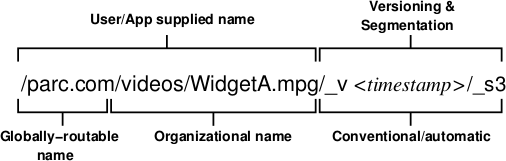
\includegraphics[width=\columnwidth/2]{Images/ndn_name.png}
\caption{NDN name schema example.}
\label{fig:ndn_name}
\end{figure}

NDN has a consumer-driven communication model, thus the receiving end in NDN is in control of communication. Two distinct packets are used to drive communication; interest and data packets. In order to query for data names in the NDN network, the interest packet is used by the consumer. When this interest packet is received by a node in the NDN network that has the data (producer), a data packet is returned. This data packets is send back over the same route as the interest packet was sent, resulting in symmetric forwarding. As discussed earlier, data may be cached on the intermediary hops in the NDN network.

NDN has an advantages over IP, it's able to use multiple paths and unlike IP it's able to handle loops at the forwarding layer. A loop-free topology is realized by inserting a nonce in every interest packet which allows to identify duplicate interests for named data, allowing multiple paths to be used which could increase throughput efficiency. Information about paths in the network are maintained in a layer called the strategy layer. This layer keeps track of two-way traffic and changes local forwarding decisions based on traffic observations. A face in NDN holds a connection to a forwarder, which could be of any class of the underlay (e.g. TCP/IP, Bluetooth or any other supported underlay).

The NDN packet forwarding engine is composed out of three data structures; The FIB, CS and PIT. The FIB is used to forward interest packets towards potential source(s) of matching data. The FIB allows a list of outgoing faces towards a single prefixes. In contrast to an IP FIB, a list for a single destination is not allowed due to network loop problems. The behavior of the forwarding can be changed by using different forwarding strategies. Before an interest packet is send out to the FIB it is first stored in the PIT along with the requesting face. An interest packet will remain in the PIT until a user defined timeout is reached, or when a matching data packet has returned from a source. The prefix and requesting face in the PIT define a return path back to the requester at each hop, this is referred to as the breadcrumbs path. The CS acts as the cache in NDN, which is used to provide the distributed property in NDN. This cache also has strategies, one for evicting data objects from the cache and one for stashing data objects in the cache.

\subsubsection{NDN strategies}
As described in section \ref{overview-ndn} there are two kinds of caching strategies; a caching decision and a cache replacement strategy. A caching decision strategy is used to determine in which router along the reverse path of an interest packet will cache the data \cite{koulouzis2018information}. The following caching decision strategies are the most well-known.

\begin{itemize}
    \item Leave copy everywhere; used to cache data object packets along each hop in the NDN path.
    \item Leave copy down; used only by the first router in the NDN path after either the original producer or an NDN cache.
    \item Leaving copies with probability; used to cache data objects with the probability of 1/(hop count).
    \item Leaving copies with uniform probability; used to cache data objects with uniform probability.
\end{itemize}

A cache replacement strategy is used to determine which data objects to evict from the cache in order to make room for new data objects. The following cache eviction strategies are the most well-known.
\begin{itemize}
    \item First in first out; used to evict the first data object that was inserted from the cache.
    \item Random replacement; used to evict random data objects from the cache.
    \item Least recently used; used to evict the least recently used data object from the cache.
    \item Least frequently used; used to evict the least frequently used data object from the cache.
\end{itemize}

The information stored in the PIT and FIB can be used to determine how to forward an interest packet out to one or more faces. These strategies are meant to give adaptive decisions based on network conditions. The following forward strategies are the most well-known.
\begin{itemize}
    \item Flooding; used to forward received interest packets towards every face, excluding the face the interest originated from.
    \item Best-route with caching; used to calculate the best path with Dijkstra's algorithm (least amount of hops) to reach a data object cache.
    \item Best-route without caching; used to only satisfy interest packets towards the original data publishers, thus excluding intermediary caches along the NDN path.
\end{itemize}

\subsection{McCabe}
\label{overview-mccabe}
As briefly described in section \ref{introduction-related-work}, McCabe's book "Network Analysis, Architecture, and Design" \cite{mccabe2010network} is about applying a systems methodology approach towards network design. McCabe's approach consists out of three core phases; analysis, architecture and design. These phases in McCabe describe how to make technology and topology decisions in a network. These decisions are guided based on inputs for the three core phases, the initial input can be from users and/or from network metrics. Consecutive processes use the output of previous processes as input, thus these processes are interconnected. In this section we will describe McCabe's method in more detail.

In figure \ref{fig:mccabe-process} the three core phases are illustrated in \textit{italic} while the processes are in normal text. In order to highlight the core phases by name they are \underline{underlined} in the figure. The first phase (analysis) has as goal to understand the network and potential problems in terms of performance and efficiency in order to determine network requirements. This is done by developing sets of problem statements and objectives that describe what the target network should address. Therefore, historical data from network management (monitoring), requirements gathered from the network users, staff and management are included in the analysis phase. Furthermore, these metrics are then compared to the relationships between users, applications, devices and other networks in order to determine if requirements match with the user and network expectations. The second and third phase (architecture and design) uses the output of the first phase to establish a high-level design of the network. This network design determines which technology and topology choices are justified to improve the network requirements established in the first phase. The fourth process is implementing the design, test if requirements are met and finally accept the implementation. These phases are intended to be iterative and by no means define a final architecture design. This is due to the fact that requirements, technology and user behaviour can change and with that the network design.

\begin{figure}[H]
\centering
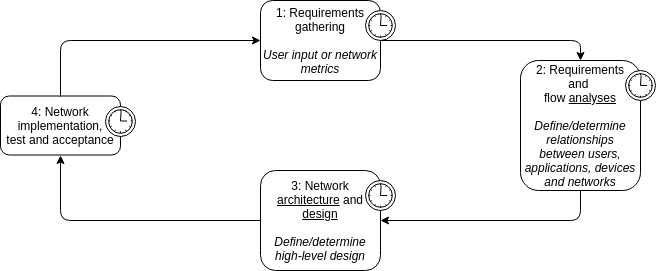
\includegraphics[width=\columnwidth]{Images/mccabe-process.png}
\caption{Cyclic and iterative nature of McCabe's processes and phases.}
\label{fig:mccabe-process}
\end{figure}

\subsection{TOSCA}
\label{overview-tosca}
% Make sure you talk about templates, not just descriptions
% Describe DRIP, OpenStack and an orchestrator in general
OASIS, an organization which is a global nonprofit consortium that works on open-standards, published the first TOSCA standard in 2014. The TOSCA standard is meant to standardize data modeling for cloud orchestration environments and applications. The latest version 1.1 \cite{tosca-standard}, was released in 2018. In this section we will highlight the important features of TOSCA, relevant to our research scope. Section \ref{planning-deploying} will merge TOSCA with McCabe's method (section \ref{overview-mccabe}).

Portability and automated management of enterprise IT infrastructures are major concerns. Infrastructures may need to run on heterogeneous components due to application needs. Having different descriptions of deployment and management for each environment complicates an infrastructure. This challenge introduces new requirements and concepts for deployment, configuration, operation and termination of components that make up an entire infrastructure. TOSCA provides a method to describe these components in generic modeling templates. In which an orchestrator can be used to implement these descriptions. Thus, TOSCA provides a single description for an entire infrastructure consisting out of templates, which is then implemented by an orchestrator. TOSCA orchestrators are e.g. DRIP and OpenStack. DRIP is currently a prototype which uses the open cloud computing interface and currently supports Amazon EC2 \cite{amazon-website}, EGI FedCloud \cite{egi-website} and ExoGENI \cite{exogeni-website} clouds. Furthermore, DRIP also supports Ansible playbooks \cite{ansible-website} for configuration management and contains a deployment agent for e.g. Kubernetes (discussed in section \ref{overview-virtualization}). This results into a portable (can be run by any orchestrator that understands TOSCA) and automated (implementation carried out by an orchestrator) method of infrastructure management. This allows interoperability and reusability of TOSCA template descriptions on different cloud providers. Seaclouds \cite{seaclouds-website} (EU FP7 funded project), not to be confused with SeaDataCloud, is already managing infrastructures based on TOSCA. Google, Red Hat, Canonical and IBM are also involved with the development of TOSCA, signifying that broader adoption may follow in the future.

TOSCA template descriptions consist out of the following core components; nodes, relationships and interfaces. Nodes can be a host, container or VM and are connected to each other through relationships such as 'dependsOn', 'hostedOn' and 'connectsTo'. These relationships can be used to describe that a VM is 'hosted on' a host (e.g. a bare metal machine). Or that a set of containers 'depend on' each other for functionality and 'connect to' e.g. a database. Such as a containerized web application that requires a database, facilitated by another container. Interfaces are used to control the life cycle of a component and consist as a set of hooks to trigger actions, these actions are create, configure, start, stop or delete. These hooks can be triggered to e.g. configure and create containers, stop or start a service or do system maintenance such as delete artifacts after a service is stopped. Furthermore, constraints can be set for the input values in these template descriptions. These can be e.g. that the amount of CPU's should be defined with integers and be should contain a value more than one. However, the orchestrator is responsible for verifying these constraints, TOSCA is merely a means to describe components in an infrastructure.

\subsection{Virtualization}
\label{overview-virtualization}
Virtualization is part of modern day infrastructures. It provides more efficient use of resources and flexibility because multiple VMs and containers can be deployed on any host that supports them. VMs are virtual operating systems that run in complete isolation from its host. Containers on the other hand share the kernel of its host and offer user-space isolation, which is relatively less isolation when compared to a VM. However, containers are more resource friendly than VMs in terms of needed compute power, memory and disk space. This section will briefly describe these two forms of virtualization.

Cloud providers such as Amazon provide easy access to compute resources, one way to access these resources is by deploying a VM on their platform. VMs and its resources can be added or removed via management interfaces or API's. This allows an infrastructure, that e.g. runs on the Amazon cloud platform, to flexibly scale in or out. Containers offer the ability to package software components together with all dependencies (e.g. libraries and binaries), such a package is called a container image. Docker is a popular platform to build and manage container-based virtualization. Once a Docker image is built it can be distributed through so-called Docker registries, such as Docker Hub \cite{dockerhub-website}. An important property of containers is that they aren't persistent, this means that containers revert back to their original image state and that data created inside the container is lost when the container has stopped or crashed. In order to make containers persistent, a data volume can be mapped onto the container's host, thus storing data outside the container. Kubernetes \cite{kubernetes-website} can be used to automate application deployment, scaling, and management of containers. In Kubernetes a container is called a pod, this may be a Docker container. These Kubernetes pods can be deployed in a cluster of Kubernetes nodes, spanning over e.g. different data centers. This offers great flexibility by packaging an application in a pod and then scale the application in or out through different data centers with Kubernetes. Kubernetes also offers high-availability features, such as automatically restart a pod when a crash occurs or load-balance requests by using a pool of identical pods in e.g. a round-robin fashion. This can be done by configuring a logical set of pods as a service. In order to custom tailor pods, environment variables can be used. These environment variables are then available inside the pod's namespace. Scripts that are executed inside the pod can then use these environment variables to setup e.g. a network configuration by specifying routes and a gateway. In Docker these scripts can be executed via a so called \texttt{ENTRYPOINT} \cite{dockerfile-reference}. NFV is a network architecture concept which uses virtualization to create and manage higher level network functions, as software, on commodity hardware. These functions may be interconnected to create a network service such as load-balancers, firewalls or intrusion detection. This architecture differs from traditional network architectures, where network functions are provided by hardware devices. NFV provides the ability to easily duplicate network functionality and expand the network locally or into other data centers. NFV is usually managed by an orchestrator to automate deployment, thus providing less overhead than traditional network management with hardware devices.
\section{Method}
\section{Results}\label{res}
If needed, we can discuss our results here, such as performance, scalability utilization, interoperability utilization
But perhaps it would be better to include a subsubsection with the results in each methodology section
\section{Discussion and experimental results}\label{disc}
%What 'advice' to give to the reader? Discuss difficulties (e.g. tosca) and such.

% include preliminary performance measurements, emphasize that it's outside the scope of our research, no real conclusions should be made, just observations, this needs to be made very clear

%Metadata, rules, web resolver link or not etc. all depending on \gls{pid} and cloud provider.


%%% ZHAO feedback
    %   - how do they work as a whole
    %   - Demonstrate its usage via example: show all components
    %   - some performance study etc?
    %   - summarize what you did
    %   - novelty (quality of being new and original)
    %   - weakness

% what is the value of this research?
% distribution of data
% deployment of ndn network by using cloud
% request pids but actually query the ndn network

% weaknesses
% only 3 pid types in poc
% not implemented full tosca deployment
% more detailed planning if more data is fed to planning method

In this section we will discuss our proposed solutions that we explored in order to answer the research questions. Furthermore, we will discuss some preliminary \gls{ndn} performance of our proof of concept in section \ref{discussion-performance}.

% RESEARCH QUESTION NDN
% How to plan and manage an NDN's life cycle with scalability in mind?

% To answer this research question we need to analyze the known scalability problems in NDN. Furthermore, the term scalability needs to apply to manageability as well. If scaling in or out in terms of resources is made uncomplicated, the efforts needed to manage this infrastructure needs to stay the same.

%     \item[--] Which \gls{ndn} scaling problems are known?
%     \item[--] Which method can be used to plan an NDN?
%     \item[--] How to deploy an \gls{ndn} with scalability in mind?



% FOLLOWING NEEDS TO BE ADDED ACCORDING TO FINAL FEEDBACK

%       first come back to the research questions and analyse how and why the questions have been solved - highlight the value that has been conveyed to the reader

%       address the needs (business) for research clouds and connect the research question to it clearly and how it's answered

%       refer back to related work (field of big science) where \gls{ndn} proved to be a success in order to improve data distribution and network efficiency

% highlight that with more users (which is expected with the growth of research clouds and their users) - the caching will come more to use

%   address that this is a general approach to the problems faced by research clouds

%   discuss that udt could potentially improve UDP-like traffic

%       "McCabe is a published method used by e.g. NASA network engineers to maintain their infrastructure" - Something along these lines, can also be in related work (the NASA part) -   But it should be clear that this is a published method to guide large deployments methodologically.

%       address that for accurate planning it is needless to say that monitoring of infrastructure is required

%       \gls{ndn} facilitates data distribution scalability, the deployment method is used to facilitate a manageable deployment. I will try to make this distinction in more detail in the discussion section.

Research clouds make large dataset availalbe to many users, with growth expected in the future. Lim et al. researched and proved the effectiveness of \gls{ndn} for big science workflows, as discussed in section \ref{introduction-related-work}. However, the data distribution benefits provided by \gls{ndn} would become unscalable without the means to maintain the life cycle. Therefore, our research developed and tested a method for planning and managing the \gls{ndn} life cycle on a larger scale by utilizing cloud providers.

The method is a general solution for planning and deploying the \gls{ndn} regardless of the research cloud its size. As demonstrated in section \ref{planning-deploying}, we have allowed the ability to flexibly scale a data distribution network. Which, with the use of the \gls{tosca} standard, could be deployed in different TOSCA-ready cloud providers without alteration. This flexibility allows the data distribution network to scale easily and make management uncomplicated. However, TOSCA-ready cloud providers are still rare, for our method to be more relevant, a wider adoption is needed.

The McCabe method \cite{mccabe2010network} is utilized to establish the requirements and high-level design of the \gls{ndn} in TOSCA. McCabe offers a proven, yet simple methodological approach for defining the design goals, which are then used to define the \gls{tosca} descriptions.

Furthermore, in research clouds identification services are used and utilize different \gls{pid} schemas. Our research created a better integration between the identification services and the data transmission services. Where traditionally IP is used for host-to-host communication, our solution utilizes NDN.


%       The work you did with NDN/PID is to investigate how identification services and transmission services can be better integrated. The current world: \gls{pid} is publication, and transmission is based on other network protocols. Our motivtion is to investigate if PID, caching, digital object discovery, routine etc. can be all implemented using the \gls{ndn} technology.



%       address that wide adoption of tosca is needed for this method, at present time this is not the case, but the research and adoption look promising

%       address that research clouds have a federated nature, while this train of thought assumes a centrally controlled method of deployment - approach this like i) as internal data-sharing platform per infrastructure, ii) as a third party data-sharing platform, one can deploy and operate for multiple infrastructure. The business model is not the key focus of the paper; but it provides technical possibility to make those servies.

% only address this part below as 'based on related work' to clearly define what the contribution was
NDN requires a different namespace format than PIDs, this is due to the incompatible nature of these namespaces. Thus a translation was needed from the \gls{pid} to the \gls{ndn} namespace, this solution was demonstrated in section \ref{pid-poc}, where we explored the possibilities of making the \gls{pid} and \gls{ndn} namespaces interoperable.

% needs to come back first to the research questions, then provide how this was answered
Therefore, the focus was on developing an extendable solution for new \gls{pid} schemas. Our solution succeeded by making use of regular expressions to match with a certain \gls{pid} type, and then call the associated function in order to do the translation to an \gls{ndn} name. Furthermore, this solution was integrated into our \gls{ndn} proof of concept. We were unable to implement our solution into the existing \gls{naas4pid} software, as this was not made publicly available.

% relate this transparcy part to a specific research question
To cache an object in our \gls{ndn} proof of concept, the user is required to first request the object from the \gls{pid} server. The object can then be requested in \gls{ndn} afterwards. Therefore, providing transparency for the user by not requiring any further user input, has not been implemented but can be achieved as described in section \ref{results-pid}. In a previous study, user input was required after translation, which is also the case in our current proof of concept. In section \ref{pid-poc} we describe how transparency for a user can be achieved. This is accomplished due to the gateway’s responsibility for \gls{pid} to \gls{ndn} translation and the object retrieval which is taken care of by the client. Our solutions are made freely available under the General Public License (GPLv3) license\footnote{\url{https://github.com/AquaL1te/rp2}}.

An alternative, less complicated design is also possible, where the client does not have to support NDN. This is accomplished by making the gateway communicate over \gls{ndn} to the \gls{ndn} and TCP/IP to the client. A client that wants to retrieve a object, uses this gateway as their resolver. The gateway retrieves the object from \gls{ndn} (or from the \gls{pid} server if it is not already in NDN) and sends this back to the client through TCP/IP. However, the gateway needs to cache the object before sending it to the client, which can cause delay for the client when retrieving an object. This design does not require the client to support \gls{ndn} as it can retrieve objects through the gateway with regular web browsers, which communicate with the gateway over HTTP. 
% (For each \gls{pid} type one gateway? So you only have to add another gateway when a new \gls{pid} type is introduced?)

% You can explain that the \gls{ndn} provides different opportunities for data infrastructures: i) as internal data-sharing platform per infrastructure, ii) as a third party data-sharing platform, one can deploy and operate for multiple infrastructure. The business model is not the key focus of the paper; but it provides technical possibility to make those servies.

% Focus on the needs and business scenarios where we need scaling, and analyze how you did can enable those scaling. Other parts will have to be left as future work.















%This is due to gateway’s responsibility for \gls{pid} to \gls{ndn} translation and the object retrieval, which is taken care of by the client.
%combining the scripts that we have created by adding a conditional statement. This statements checks whether an object is already published in NDN.

% The second problem statement has been addressed in section \ref{planning-ndn}, where \gls{ndn} was identified as a potential solution for the data distribution and network load problem. Therefore, a method of planning and deploying such a network was explored in detail and tested. It was concluded that a scalable and manageable data distribution network can be realized by using a NVF-style of an \gls{ndn} deployment. Of which the life cycle can be managed by the use of \gls{tosca} templates. However, a full \gls{tosca} orchestrated deployment could not be demonstrated. This was due to the fact that \gls{tosca} orchestrators are still in development. However, Kubernetes was used as a substitution to demonstrate the deployment level on a higher level in the deployment chain. In practice, Kubernetes would be deployed by a \gls{tosca} orchestrator as well. Compared to traditional network management, NVF provides more flexibility, by the use of a centrally control the virtual \gls{ndn} functions in the network. If the behavior of the users change and thus the stress on the network, our solution will be able to adjust the network without adding extra complexities.





%Discussion or future work.
% For our proof of concept we created two scripts for the client side and two scripts for the gateway to demonstrate our design. The gateway and client are conceptually part of the \gls{ndn} network we have setup with Kubernetes and can be scaled in or out. The responsibility of the scripts on the client side is to retrieve a requested object either from the \gls{pid} server or from NDN. The scripts that are implemented in the gateway send either the \gls{pid} link or the name in \gls{ndn} to the client for retrieval of the requested object after translation. This depends on the object being published in \gls{ndn} or not.

%Usually, \gls{ndn} operates with in-network caching. However, we used \texttt{ndnputchunks} to cache objects in \gls{ndn} in our proof of concept, which does not serve a file but works with a standard input stream. Data is cached in-memory and takes up to three times the size of the object for encoding \cite{ndnput-mem}. For using a persistent file cache we already compiled the base image of our proof of concept with repo-ng\footnote{https://github.com/named-data/repo-ng} as that utilizes
%is part 
%the NDN-CXX application we already use. Repo-ng is an open source project and is used to set up a data repository for a persistent file cache.

% For supporting multiple \gls{pid} types, we demonstrated the use of three \gls{pid} types in our proof of concept. This already proves that supporting multiple \gls{pid} types is possible. Adding more \gls{pid} types to our proof of concept, such as the ones described in Karakannas' research \cite{icn-bd} is possible but we see this more as work for an implementation.

%TCP \gls{pid} part still has to be adjusted to new \gls{pid} server. 
%> Done
%"NDN is not designed for retrieving data objects with big sizes", as Zhao stated. 
%It is meant for "large datasets" (which could be a lot of small files) and not "large objects". 
%Maybe that's why we don't see that much of a difference between \gls{ndn} vs TCP/IP for a 1000MB object in comparison to \gls{ndn} vs TCP/IP for a 100MB object... 
%Should we also state this and remove the 1000MB benchmark and run some benchmarks with a 10MB file? 
%> Done
%First time is not taken into account. So results are based on direct link between consumer and router where the data is cached.

\subsection{Preliminary performance measurements}
\label{discussion-performance}
In this section we will briefly discuss the preliminary performance of our \gls{ndn} with \gls{pid} interoperability proof of concept. The results gathered were merely based on best-effort test scenarios and are inconclusive. Therefore, further and more detailed research is required, which we will discuss in more detail in future work (section \ref{fut}). 


We used for both TCP/IP and \gls{ndn} the default values.
For TCP/IP, we did not tweak the \gls{mtu} values and kept the TCP parameters to their defaults, such as the default Linux TCP congestion algorithm; Cubic. For the TCP/IP benchmarks we used the the \texttt{urllib.request} Python module, which uses the HTTP 1.1 protocol over TCP \cite{urllib}. For NDN, we used the default MTU setting when creating a face (8800) with \texttt{nfdc} (part of the NDN-CXX application) and did not tweak any of the parameters, which are highlighted in section \ref{fut}. For publishing objects in NDN, we used the default settings of \texttt{ndnputchunks}, which has a MTU of 4400. The underlying technology is still IP in NDN. However, \gls{ndn} uses hop-by-hop fragmentation. This technology enables fragmentation at each hop if needed. Which means that the whole network no longer needs to limit its MTU size to the smallest denominator \cite{ndn-mtu}.
% We want to highlight that the results we present in figure \ref{fig:perftest-1} and \ref{fig:perftest-2} are preliminary. A range of parameters can be used to optimize \gls{ndn} network performance.

The architecture used in our experiments is as follows. The \gls{ndn} consumer and router container reside on 'nimes', while the \gls{ndn} producer and router reside on 'mulhouse'. Furthermore, they are interconnected via the internet, using the Kubernetes overlay network as shown in section \ref{planning-architecture} figure \ref{fig:high-level-network-design}. As the connection is routed over the internet, latency can occur as it depends on the path a packet takes. The tool \texttt{traceroute} shows that there are no intermediate hops between 'nimes' and 'mulhouse'. The disk throughput of the server where the containers reside has a write speed of 180MB/s. Network latency is around 200 microseconds, measured by the tool \texttt{arping}.
The preliminary performance results of our Handle \gls{pid} server and the \gls{ndn} are illustrated in boxplots (figure \ref{fig:perftest-1}, \ref{fig:perftest-2}, \ref{fig:perftest-3}, \ref{fig:perftest-4} and \ref{fig:perftest-5}). We ran the following performance tests within our proof of concept using a 10MB, 100MB, 250MB, 500MB and a 1000MB data object. We performed the performance tests ten times for each object size and protocol and are processed in the illustrated boxplots. The different object sizes were chosen in order to determine if there is a certain trend between the object size and performance. This performance trend is illustrated in figure \ref{fig:perftest-6} and shows the average of the test runs. We can observe that \gls{ndn} over UDP outperforms the TCP/IP connection used for retrieving data objects from the Handle \gls{pid} server that we setup with all chosen object sizes. Furthermore, \gls{ndn} over TCP outperforms \gls{ndn} over UDP. This result correlates with the research done by Lim et al., as discussed in section \ref{introduction-related-work-ndn}. The line chart shown in figure \ref{fig:perftest-6} shows that the lines converge after the 250MB mark. Which means that the relative difference between \gls{ndn} and TCP/IP becomes smaller with object sizes bigger than 250MB. This is due to NDNs nature of handling big object sizes. These can cause a performance problem, because the cost of retransmission when interests are retransmitted (or re-issued) becomes unsustainably high \cite{ndn-objects}. % Their research concludes that \gls{ndn} provided performance improvements compared to classical climate data delivery techniques based on TCP/IP. In addition to this, \gls{ndn} over TCP demonstrated a more reliable and faster performance due to the allowance of larger dynamic window sizes and congestion control.

\begin{figure}[H]
\centering
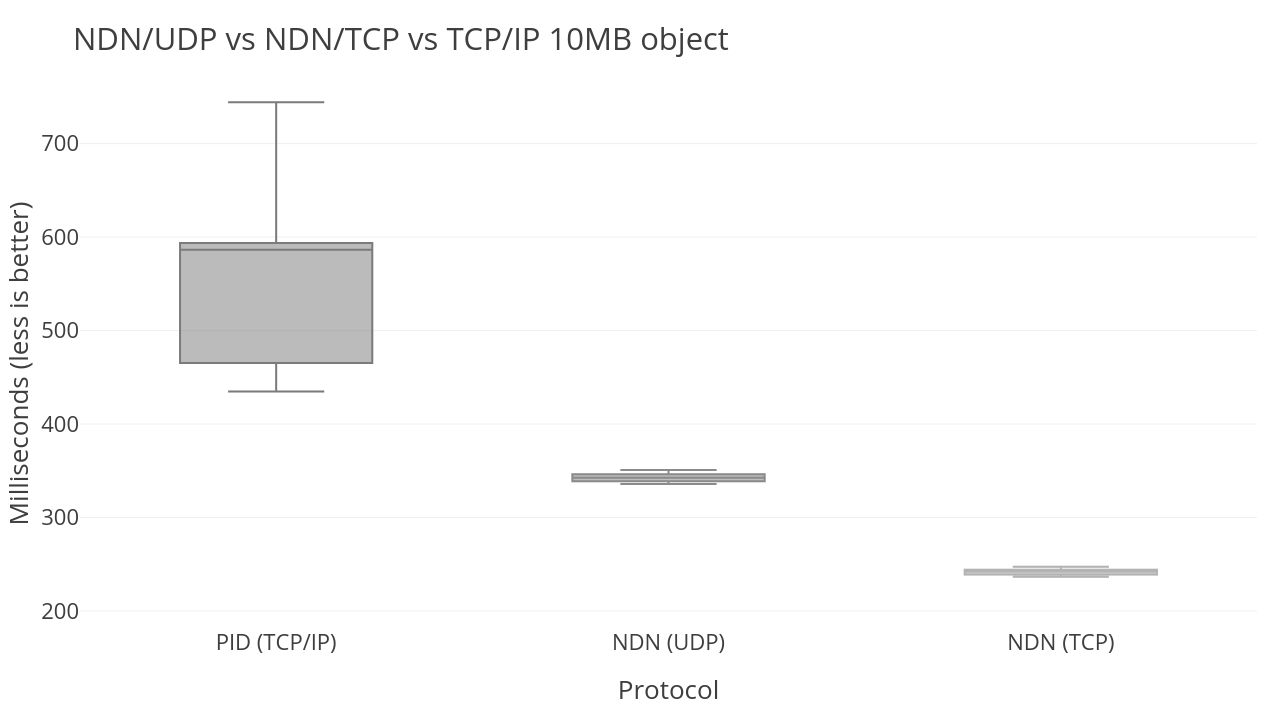
\includegraphics[scale=0.43]{Images/bench10MB_grey.png}
\caption{Performance test TCP/IP vs \gls{ndn} with a 10MB object.}
\label{fig:perftest-1}
\end{figure}

\begin{figure}[H]
\centering
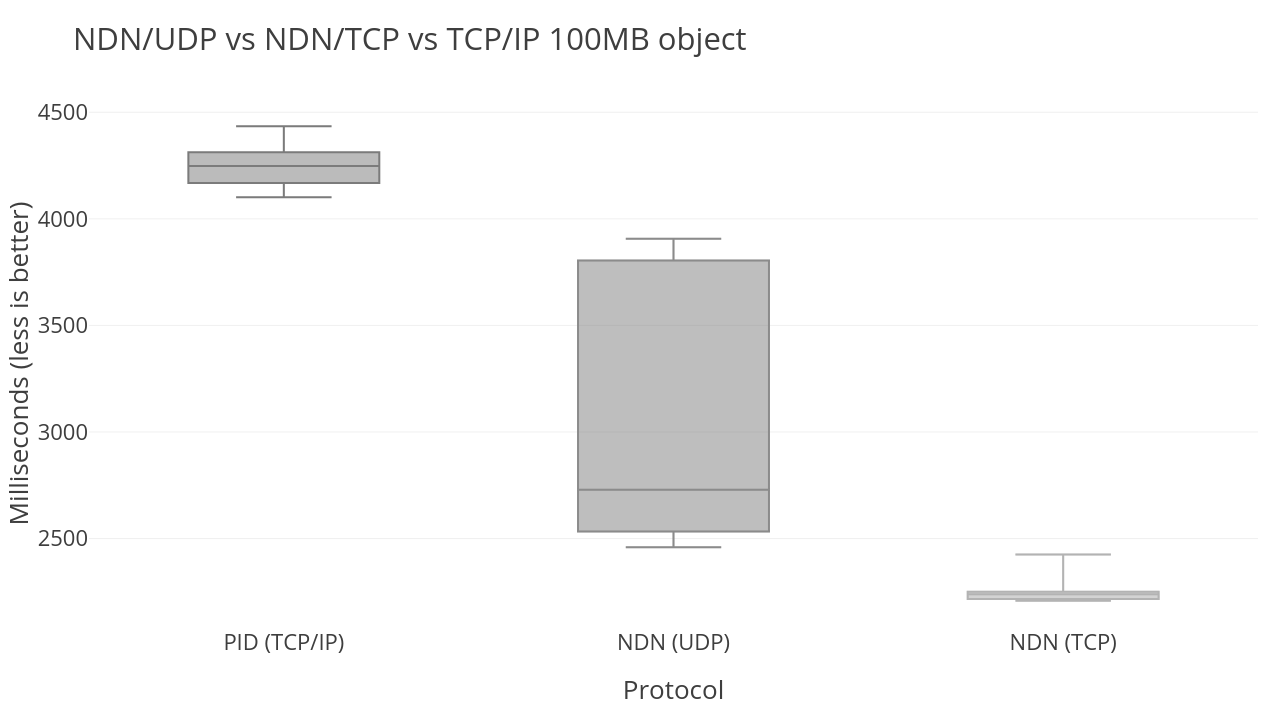
\includegraphics[scale=0.43]{Images/bench100MB_grey.png}
\caption{Performance test TCP/IP vs \gls{ndn} with a 100MB object.}
\label{fig:perftest-2}
\end{figure}

\begin{figure}[H]
\centering
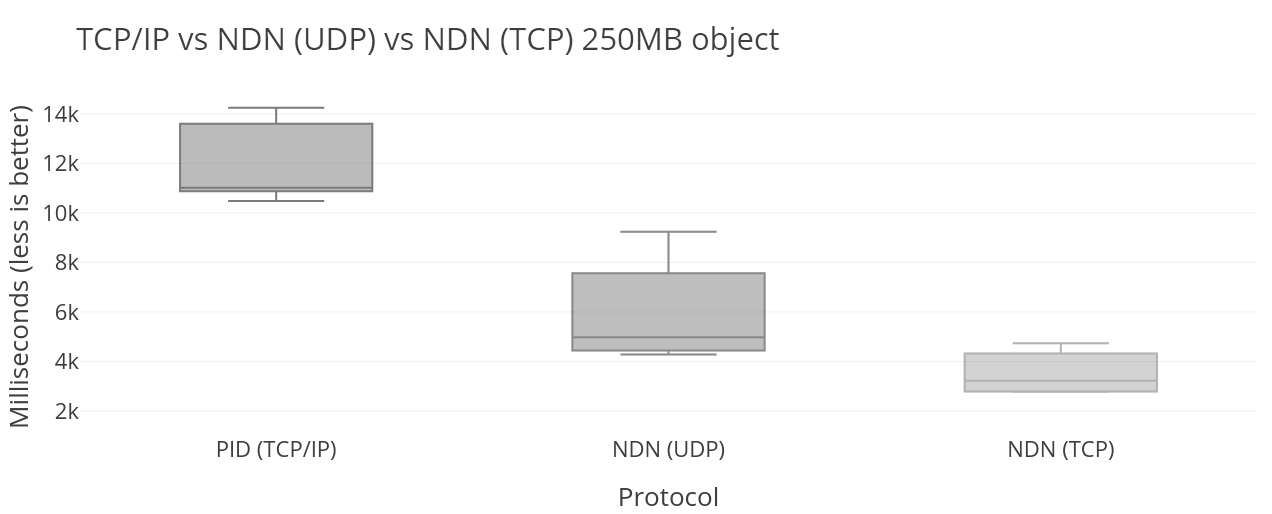
\includegraphics[scale=0.43]{Images/ndn_tcpip_250_grey.png}
\caption{Performance test TCP/IP vs \gls{ndn} with a 250MB object.}
\label{fig:perftest-3}
\end{figure}

\begin{figure}[H]
\centering
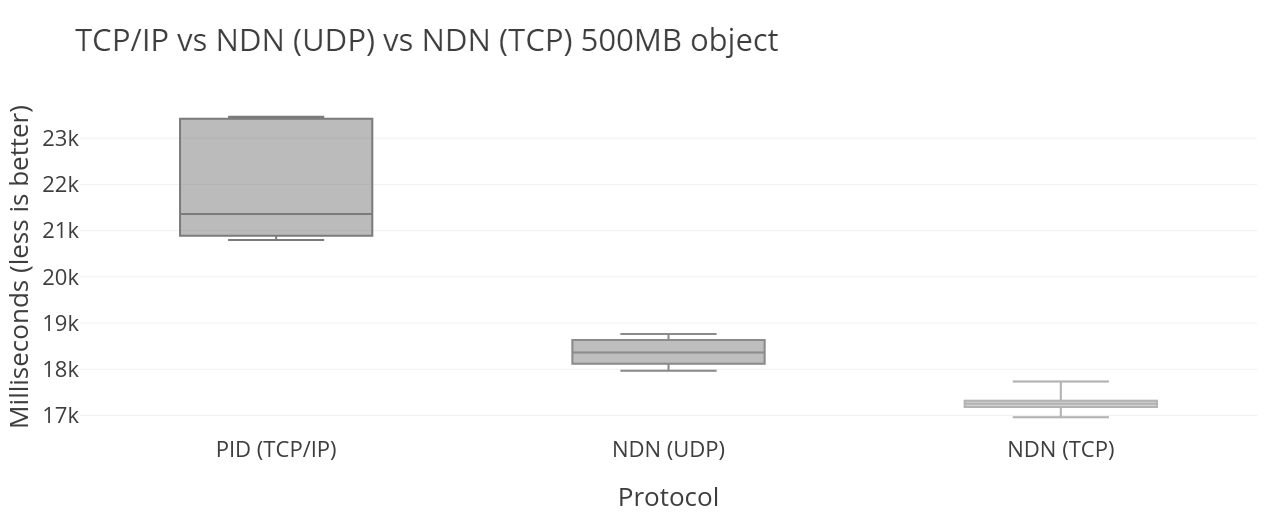
\includegraphics[scale=0.43]{Images/ndn_tcpip_500_grey.png}
\caption{Performance test TCP/IP vs \gls{ndn} with a 500MB object.}
\label{fig:perftest-4}
\end{figure}

\begin{figure}[H]
\centering
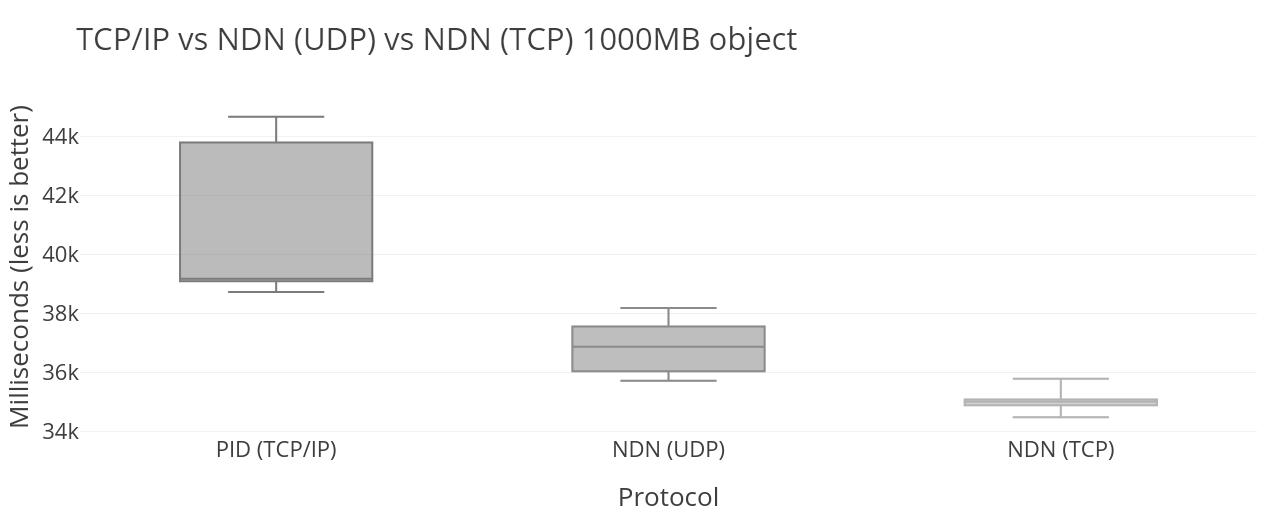
\includegraphics[scale=0.43]{Images/ndn_tcpip_1000_grey.png}
\caption{Performance test TCP/IP vs \gls{ndn} with a 1000MB object.}
\label{fig:perftest-5}
\end{figure}

\begin{figure}[H]
\centering
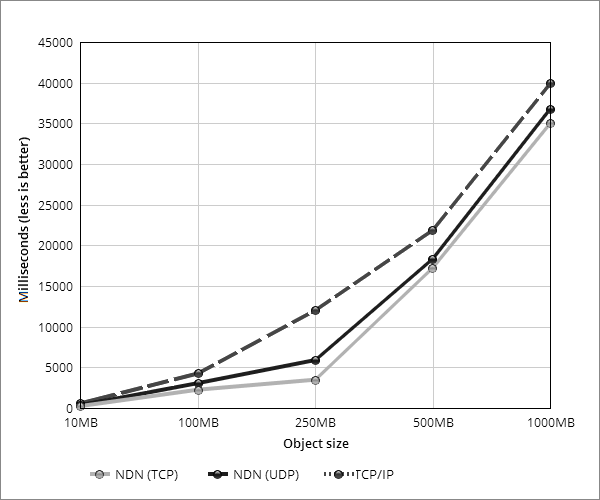
\includegraphics[scale=0.7]{Images/linechart5.png}
\caption{Object size to performance relation.}
\label{fig:perftest-6}
\end{figure}

When observing the results, we can see that it takes roughly more than four seconds to retrieve a 100MB object over TCP/IP, which does not seem to be optimal. 
%is not optimal as a 1Gbps Ethernet connection is used for the benchmarks. 
It seems that our Handle \gls{pid} server, which is set up with \texttt{cordra-1.0.7} software is the bottleneck. Since we got faster results when retrieving the Linux kernel for example. We can retrieve a 102MB Linux kernel\footnote{https://cdn.kernel.org/pub/linux/kernel/v5.x/linux-5.2.8.tar.xz} in ${\sim}1$ second within a container in our proof of concept. This seems to be faster than the default \texttt{ndnputchunks} settings with a MTU of 4400. When raising the MTU to 8800 for publishing a object in \gls{ndn} with \texttt{ndnputchunks}, to reduce the number of signatures needed to transmit a object, we can observe that the average time to retrieve an object through \gls{ndn} takes less than a second (${\sim}850$ milliseconds). 
When retrieving a object over \gls{ndn} UDP with a MTU set to 8800 in \texttt{ndnputchunks}, we cannot observe any difference with our results shown in figure \ref{fig:perftest-2} with a MTU of 4400 over \gls{ndn} UDP. This may be caused by UDP's limitations in \gls{ndn} as described in section \ref{introduction-related-work-ndn}. 

%However, in this case we tweaked the default \texttt{ndnputchunks} settings for publishing a file in NDN, but the default face settings are already set on 8800 when creating a face.


% TO-DO: 
% - Mention \gls{tosca} difficulties.
% - Preliminary benchmark results (PID server on nimes)
% high-availability kubernetes + persistent volumes + ndn cache
\section{Conclusion}\label{conc}
In this research we present a design for sharing digital objects using NDN with support for multiple PID providers. Our findings give insight for distributed infrastructures that manage large and diverse sets of data like SeaDataCloud and CS3. 

First, we started researching the state of the art technologies for creating our design. After, we discuss the methods for used for our design. The first method manages to achieve PID interoperability of different PID types with the NDN namespace. While the second method covers planning and scaling of an NDN network. 

The first method in section \ref{pid-poc} showed that our principles regarding PID interoperability with the NDN namespace can be adhered. Metadata can be parsed to fill in possible naming gaps in an NDN name. However long NDN names have to be taken in account, as that can degrade performance. 
%Translation of PIDs to an NDN name can be made transparent to the user, as the gateway is responsible for the translation and the client takes care of object retrieval either from the PID provider or from the NDN network.
Our solution is designed to be extensible, new PID schemas can be added at the gateway. Therefore, only the gateway needs to update its PID support in our design. The client is agnostic towards PID types, it is up to the gateway to verify the types and send an appropriate response. This elevates the burden of updating client software.

The second method in section \ref{planning-ndn} achieves flexible scaling and planning of an NDN network by managing the NDN infrastructure with Kubernetes. We have demonstrated a method for scaling in or out the NDN application, despite lacking a orchestrator like DRIP to demonstrate scaling in or out resources to other cloud providers with TOSCA. Our method allows to reconfigure an NDN infrastructure 
by interacting with Kubernetes as the orchestrator.
%Mention TOSCA again and that we conclude that TOSCA can be used.
We concluded that a scalable and manageable data distribution network can be realized by using a VNF-style of an NDN deployment. 

Finally, we discuss preliminary performance measurements. Our results show that NDN over TCP gives the best performance, which correlate with previous work.

%This research investigated sharing digital objects using NDN, where we achieved PID interoperability of different PID types with the NDN namespace and planning and scaling of such an NDN network. 
%Our findings give insight for distributed infrastructures that manage large and diverse sets of data like SeaDataCloud and CS3. We 

%explain why NDN networking should be chosen for retrieving digital objects instead of host-to-host communications.

%The implementation of our design in a proof of concept shows that our principles regarding PID interoperability with the NDN namespace can be adhered. The translation of PIDs to an NDN name can be made transparent to the user, as the gateway is responsible for the translation and the client takes care of object retrieval either from the PID provider or from the NDN network. Only a PID should be needed from the user input. Translation is achieved by first recognizing the PID type based on pattern matching and then hierarchically divide the PID to an NDN name. 

%Our solution is designed to be extensible, new PID schemas can be added at the gateway. Therefore, only the gateway needs to update its PID support. The client is agnostic towards PID types, it is up to the gateway to verify the types and send an appropriate response. This elevates the burden of updating client software.

%Support for multiple PID types is also realized by adding the schema of the PID types at the gateway, which makes it also easily extensible to support future PID types. Adding PID types at the gateway overcomes the hurdle of updating the client side with the schema of the new PID type each time when a new PID type is introduced.

%We achieved flexible scaling and planning of an NDN network by managing the NDN infrastructure with Kubernetes. We have demonstrated a method for scaling in or out the NDN application, despite lacking a orchestrator like DRIP to demonstrate scaling in or out resources to other cloud providers with TOSCA. Our method allows to reconfigure an NDN infrastructure by interacting with Kubernetes as the orchestrator. The YAML configuration of Kubernetes can be seen as the TOSCA template description which is processed by Kubernetes, which in turn acts as an orchestrator instead of DRIP.
\section{Conclusion and future work}
\label{fut}
\label{conc}
% - TOSCA blueprints are conceptual X
% - The VM and Kubernetes was deployed manually X
% - Full implementation developed needed with an orchestrator such as e.g. DRIP X
% - NDN is still experimental X
% performance tweaks that require source code changes not implemented, up for upstream.

% add the part about caching strategies and why we used the general recommendation and not the one for big data
% Initially, we started researching the state of the art technologies for creating our design. We came to the conclusion that NDN would fit the technical challenges we had to work out.
% After, we started researching \gls{pid} interoperability with the NDN namespace and found out that our principles can be adhered as discussed in section \ref{pid-poc}.



% You can explain that a detailed analysis on the NDN caching strategies and data infrastructure sharing patterns need future analysis. This is yet investigated by the thesis. You can leave it as a future work.


% NEW AND FINAL FEEDBACK - KEES
% highlight the merging of the 2 projects in conclusion

% highlight that the method needs to be tested in large scale deployment to evaluate it in practice





Our research investigated solutions for the increasing trend of data producers and consumers in research clouds. Our methods are designed to be used for large research clouds. However, the methods were only tested in a small scale proof of concept. Therefore, further experimentation is needed on a larger scale to fully prove our methods. Furthermore, data producers and consumers can make use of different \gls{pid} standards, in order to retrieve this data by name in NDN, a compatible translation was needed between these namespaces. The solution we developed for this problem is designed to be easily extensible for new \gls{pid} types. 

Research clouds are in general a federated cloud, where each federation is responsible for its own budget and infrastructure. However, our solution assumes central control over the NDN. Our solution could be approached in several ways. The solutions could be deployed as an internal data-sharing platform per infrastructure and interconnect those NDNs, thus maintaining the federated model. Or, it could be deployed as a third party data-sharing platform, where one can deploy and operate the NDN for multiple infrastructures. Our research did not explore these subjects. However, it provides the technical possibilities to deploy these solutions in such a manner.

% ANAS - SOME CONCLUSIONS SUMMERIZED ABOUT THE PEFORMANCE MEASUREMENTS - IS NDN PROMISING OR NOT? FURTHER RESEARCH IS DISCUSSED BELOW

% We have developed a method of deployment to make NDN scalable from a single infrastructure description. This was done by utilizing the properties of TOSCA templates, cloud and virtualization techniques. Furthermore, data producers and consumers can make use of different \gls{pid} standards, in order to retrieve this data by name in NDN, a compatible translation was needed between these namespaces. The solution we developed for this problem is designed to be easily extensible for new \gls{pid} types.

% presented a method and design for sharing digital objects using NDN with support for multiple \gls{pid} providers. Our findings give insight for distributed infrastructures that manage large and diverse sets of data such as SeaDataCloud and CS3.

Based on our findings we acknowledge the following subjects for further research. As described in section \ref{overview-tosca}, TOSCA orchestrators are still in development. Therefore, more experimentation is needed when these orchestrators become more mature. This can give more insight in the flexibility and utilization of these orchestrators. As discussed in section \ref{planning-poc}, due to the nature of Kubernetes, pods are deployed based on the resource requirements of a pod and the resource availability inside a cluster. Pods that run NDN functions are not only interested in Kubernetes resources, but their true value is mainly determined on locality. This is due to the distributed nature of NDN, which depends on in-network caching along the network path between data producers and consumers. If Kubernetes doesn't deploy a pod where NDN resources are needed, then human intervention is needed to specify on which Kubernetes node a pod must run. Therefore, if Kubernetes could be extended with the intelligence of also NDN's resource needs, it could deploy pods automatically in a certain geographical area in order to increase cache hits. Furthermore, the NDN faces were configured manually as well, this was due to the lack of mature NDN routing protocols. However there are two promising routing protocols in development; \gls{ospfn} by Lan Wang et. al. \cite{ndn-ospfn1, ndn-ospfn2} and \gls{nlsr} \cite{nlsr}. With a routing protocol, the NDN management process would become less complicated and more resilient.

Some NDN performance issues were identified in related work, such as when using UDP and the use of long names - mention UDT as future work for integration with NDN since UDP in NDN does not utilize congestion and flow control mechanisms.

Furthermore, metadata can be parsed to fill in possible naming gaps in an NDN name. An NDN name is unbounded, however, the length of NDN names have to be taken into account since long NDN names can degrade performance (as discussed in section \ref{introduction-related-work-ndn}). So et al. researched and developed a solution for fixed lookup times. However, this research was not made public. Integrating such a solution could prove valuable for NDN performance. Lastly, we discussed preliminary performance measurements based on a best-effort testing scenario. Our results show that NDN over TCP gives the best performance in comparison to NDN over UDP, which correlates with related work.

Furthermore, more performance measurements and analyses is needed to gather a better profile of NDN scalability with cloud resources. The performance results we discussed in section \ref{disc} are preliminary. We recommend the following test scenarios. Performance can be improved with the use of different MTU sizes (this can be configured when creating a face, as well as with the \texttt{ndnputchunks} tool) and configuring congestion threshold and pipeline types (for example fixed, Cubic or AIMD for configuring window sizes). Where the latter can also be configured when using the \texttt{ndnputchunks} tool. Furthermore, the NDN can be configured to use TCP or UDP, which can also be configured when creating a face. We recommend running different tests with the aforementioned parameters with multiple consumers in order to determine when congestion occurs. The parameters can also be combined with the most optimal NDN caching mechanism and the most optimal ordering method \cite{koulouzis2018information} to run benchmarks. These performance tests would be interesting by running it in a cloud environment, where resources can be scaled up and down.

% This part needs some tweaking maybe (already tweaked it a bit)
%For benchmarking, the tool ndn-traffic-generator\footnote{https://github.com/named-data/ndn-traffic-generator} can be used to generate random interest and data traffic in an NDN network. Although this tool only allows a fixed pipeline size (\texttt{X} amount of packets per second) and does not implement congestion control. Thus it is not very useful when comparing against TCP/IP \cite{ndnput-mem}. The tool \texttt{ndncatchunks} that we used in our proof of concept for requesting objects from NDN, is a more realistic scenario than generating random traffic as this does incorporates congestion control, which makes it more useful for comparing against TCP/IP.

The \gls{pid} interoperability solution we developed exists outside of the NDN source code. For the best application of this functionality, we recommend the integration of these interoperability functionalities into the native NDN source code. This would remove the need to run a translation gateway.

% Implementing routing protocols for NDN in our proof of concept is also worth testing. As in  our proof of concept, we manually configure all the routes.

% Lan Wang et. al. \cite{ndn-ospfn1} designed and performed a feasibility assessment in 2011 of an OSPF extension for NDN that they call "OSPF-N". OSPF-N is a routing protocol based on the existing OSPF protocol that operates on the network layer for IP networks. OSPF-N uses new types of opaque LSA's to carry NDN routing information. By using the OSPF-N configuration manager at each NDN node, it configures links to other NDN nodes, name prefixes of the content store, and the maximum number of hops to be calculated for each name prefix in order to support multipath routing \cite{ndn-ospfn2}. NLSR is also a routing protocol designed for NDN, in addition to OSPF-N. The initial design for NLSR was developed in 2013. The protocol operates at the application layer similar to existing IP routing protocols such as RIP and BGP. This protocol calculates the routing table using link-state or hyperbolic routing. Furthermore, it produces multiple faces for each reachable name prefix in a single authoritative domain .

\printbibliography

\end{document}
